\documentclass[11pt,a4paper]{article}
\usepackage[margin=2.2cm]{geometry}
\usepackage{amsmath,amssymb}
\usepackage{graphicx}
\usepackage{booktabs}
\usepackage{array}
\usepackage{enumitem}
\usepackage{xcolor}
\usepackage{listings}
\usepackage{caption}
\usepackage{fancyhdr}
\usepackage[hidelinks]{hyperref}

\definecolor{codebg}{RGB}{246,246,246}
\definecolor{kw}{RGB}{0,60,160}
\definecolor{cm}{RGB}{90,120,90}
\definecolor{st}{RGB}{150,60,30}
\lstset{
  language=Python, basicstyle=\ttfamily\footnotesize,
  keywordstyle=\color{kw}\bfseries, commentstyle=\color{cm}\itshape,
  stringstyle=\color{st}, backgroundcolor=\color{codebg},
  frame=single, framerule=0.3pt, breaklines=true, showstringspaces=false,
  numbers=left, numberstyle=\tiny\color{gray}, numbersep=6pt,
  aboveskip=6pt, belowskip=6pt, columns=fullflexible
}
\lstdefinestyle{output}{language={}, basicstyle=\ttfamily\footnotesize,
  backgroundcolor=\color{codebg}, frame=single, framerule=0.3pt,
  numbers=none, breaklines=true}

\pagestyle{fancy}
\fancyhf{}
\fancyhead[L]{ED408 -- Statistical Machine Learning II Lab}
\fancyhead[R]{Module I}
\fancyfoot[C]{\thepage}

\newcommand{\labsection}[1]{\subsection*{#1}}

\begin{document}

% ============================ COVER ============================
\begin{titlepage}
\centering
\vspace*{1.5cm}
{\Large \textbf{Indian Institute of Technology Roorkee}}\\[0.6cm]
{\large Department of Design}\\[2.2cm]
{\LARGE \textbf{ED408: Statistical Machine Learning II Lab}}\\[0.4cm]
{\large (0--0--3--1.5)}\\[1.2cm]
{\Large \textbf{Lab File --- Module I}}\\[0.3cm]
{\large Overview of Machine Learning Techniques}\\[2.0cm]
\begin{tabular}{ll}
\textbf{Dataset used:} & Berkeley Segmentation Dataset (BSDS500)\\[2pt]
\textbf{Task:}         & Boundary vs non-boundary pixel classification\\[2pt]
\textbf{Experiments:}  & 1--7 \\[2pt]
\textbf{Submitted by:} & Ayush Dhar Dubey \\[2pt]
\textbf{Programme:}    & B.Tech (Third Year) \\[2pt]
\textbf{Session:}      & 2026--27 (Autumn)\\
\end{tabular}
\vfill
{\small The complete executable programs are maintained digitally on GitHub;\\
this file records the important code sections, outputs and analysis.}
\end{titlepage}

% ============================ COMMON PRELIMINARY ============================
\section*{Common Dataset and Preprocessing (used by all experiments)}
\textbf{Dataset.} The \emph{Berkeley Segmentation Dataset} (BSDS500): 500 natural images, each hand-segmented by approximately five human annotators, with the dataset's own train/test image split. All seven Module-I experiments run on a single machine-learning problem derived from it: \textbf{given 17 hand-crafted local features of a pixel, predict whether humans marked an object boundary at that pixel.}

\textbf{Label construction (consensus labelling).} Human annotators disagree, so labels are built conservatively: a pixel is labelled \emph{boundary} only when $\geq 2$ annotators drew a boundary within $1$ px of it; \emph{non-boundary} only when \emph{no} annotator marked within $2$ px; all remaining (ambiguous) pixels are excluded. This is a deliberate label-noise control.

\textbf{Features (17 per pixel).} CIELAB colour $(L,a,b)$; Gaussian gradient magnitude at $\sigma\in\{1,2,4\}$; local standard deviation at $\sigma\in\{1,2,4\}$; $|$Laplacian of Gaussian$|$ at $\sigma\in\{1,2\}$; oriented derivative energy at $0^\circ/45^\circ/90^\circ/135^\circ$ ($\sigma{=}2$); the two structure-tensor eigenvalues (edge/corner energy).

\textbf{Why this is not a toy problem.}
\begin{itemize}[nosep]
  \item \textbf{Class imbalance:} true boundary prevalence in an image is only $\sim$2--5\%; negatives are subsampled to a $73{:}27$ ratio, preserving the imbalance story while keeping training tractable.
  \item \textbf{Heavy-tailed features:} gradient and Laplacian responses have extreme right tails (high-contrast edges), which stresses Gaussian assumptions (Exp.~3) and classical outlier rules (Exp.~6).
  \item \textbf{Correlated features by design:} the same physical edge fires many filters at once --- directly relevant to PCA (Exp.~5), the Naive-Bayes independence assumption (Exp.~3) and tree importances (Exp.~2).
  \item \textbf{Leakage-safe protocol:} train and test pixels come from \emph{disjoint images} (80 train / 30 test images; up to 160 boundary $+$ 440 non-boundary pixels per image; 8-px border excluded) --- the image analogue of avoiding temporal leakage.
\end{itemize}

\textbf{Evaluation protocol.} $48{,}000$ training and $18{,}000$ test pixels, boundary rate $26.67\%$ in both. All standardisation, fences and model selection use \emph{training} data only.

\begin{lstlisting}
# label policy (extract_bsds.py)
for g in annotators:
    votes  += binary_dilation(g.Boundaries, iterations=1)
    anymark |= binary_dilation(g.Boundaries, iterations=2)
positive = votes >= 2          # consensus boundary
negative = ~anymark            # no annotator anywhere near
# ambiguous pixels (the rest) are excluded

# per-pixel features: colour + multi-scale filter bank (17 total)
lab = rgb2lab(img); L = lab[...,0]
gradmag_s = gaussian_gradient_magnitude(L, sigma)      # sigma in {1,2,4}
localstd  = sqrt(gauss(L**2,s) - gauss(L,s)**2)        # local contrast
abslap    = abs(gaussian_laplace(L, sigma))            # sigma in {1,2}
orient_th = abs(cos(th)*gx + sin(th)*gy)               # 4 orientations
st_eig1,2 = eigenvalues(structure_tensor(gx, gy))      # edge/corner energy
\end{lstlisting}

\newpage
% ============================ EXPERIMENT 1 ============================
\section*{Experiment No.: 01}
\labsection{Title: k-Nearest Neighbours Classifier from Scratch}

\labsection{Aim}
Implement the k-Nearest Neighbours (k-NN) classifier from scratch (without \texttt{sklearn.neighbors}) and test it on BSDS500 boundary-pixel classification.

\labsection{Problem Statement}
Given the 17 standardised local features of a pixel, predict whether it lies on a human-marked boundary using only the labels of the $k$ most similar pixels in the training set. Study (i) the effect of feature scaling, (ii) the choice of $k$, and (iii) majority voting versus distance-weighted voting.

\labsection{Algorithm}
\begin{enumerate}[nosep]
  \item Standardise all features using training-set mean $\mu_j$ and standard deviation $\sigma_j$: $z_{ij}=(x_{ij}-\mu_j)/\sigma_j$.
  \item For a batch of query pixels $Q$, compute all pairwise Euclidean distances in one vectorised step using $\lVert q-x\rVert^2 = \lVert q\rVert^2 - 2\,q^\top x + \lVert x\rVert^2$.
  \item For each query, select the $k$ smallest distances with \texttt{np.argpartition} (an $O(n)$ partial sort).
  \item Majority vote: $\hat p = \frac{1}{k}\sum_{i\in N_k} y_i$. Distance-weighted vote: $\hat p = \sum_i w_i y_i / \sum_i w_i$ with $w_i = 1/(d_i+\varepsilon)$.
  \item Predict \emph{boundary} if $\hat p \ge 0.5$.
  \item Repeat over $k\in\{1,3,5,9,15,25,41,61,101\}$ and select $k$ by the validation F1-score of the boundary class.
\end{enumerate}

\labsection{Program (important sections)}
\begin{lstlisting}
class KNNScratch:
    def __init__(self, k=5, weighted=False):
        self.k, self.weighted = k, weighted

    def fit(self, X, y):
        self.X, self.y = np.asarray(X, float), np.asarray(y)
        return self

    def _dist(self, Q):                       # full pairwise matrix, no loops
        d2 = (Q**2).sum(1)[:,None] - 2*Q @ self.X.T + (self.X**2).sum(1)[None,:]
        return np.sqrt(np.maximum(d2, 0))

    def predict_proba(self, Q, batch=1000):   # batched to bound memory
        out = np.empty(len(Q))
        for s in range(0, len(Q), batch):
            D   = self._dist(Q[s:s+batch])
            idx = np.argpartition(D, self.k, axis=1)[:, :self.k]
            labels = self.y[idx]
            if self.weighted:
                w = 1.0 / (np.take_along_axis(D, idx, 1) + 1e-9)
                out[s:s+batch] = (w*labels).sum(1) / w.sum(1)
            else:
                out[s:s+batch] = labels.mean(1)
        return out
\end{lstlisting}
Key parameter settings: stratified subsample of $6{,}000$ train / $2{,}000$ test pixels (k-NN is $O(nm)$ per query); $\varepsilon = 10^{-9}$; threshold $0.5$.

\labsection{Output and Analysis}
\textbf{Program execution:}
\begin{lstlisting}[style=output]
Unscaled  acc: 0.7834
Scaled    acc: 0.8089
Best k=5 (distance-weighted): acc = 0.7964, F1(boundary) = 0.5808
Execution Status: Successfully Executed
\end{lstlisting}

\begin{figure}[h]\centering
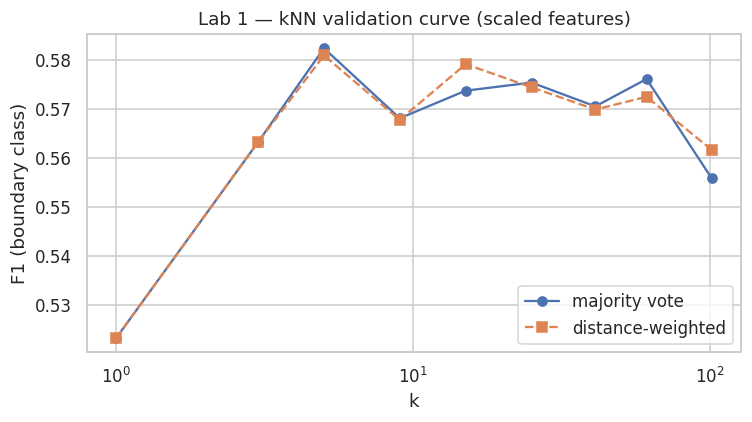
\includegraphics[width=0.72\textwidth]{figs/fig1_knn_curve.png}
\caption{Validation curve for k-NN: F1 of the boundary class versus $k$ (log scale), majority vs distance-weighted voting.}
\end{figure}

\textbf{Parameter modification:}
\begin{center}\footnotesize
\begin{tabular}{@{}clllllp{3.4cm}@{}}
\toprule
S.No. & Parameter & Original & Modified & Original result & Modified result & Observation\\
\midrule
1 & Feature scaling & standardised & raw features & acc $=0.8089$ & acc $=0.7834$ & Unscaled distances are dominated by the L channel (range 0--100) and large-$\sigma$ filters.\\
2 & Neighbours $k$ & $5$ & $1$ & F1 $=0.5808$ & F1 $=0.5233$ & $k{=}1$ overfits annotator noise near ambiguous edges.\\
3 & Neighbours $k$ & $5$ & $101$ & F1 $=0.5808$ & F1 $=0.5616$ & Very large $k$ oversmooths; thin boundary structures are voted away by bulk texture pixels.\\
\bottomrule
\end{tabular}
\end{center}

\textbf{Conclusion.} Scaling fixes the metric geometry. Unlike diffuse tabular problems, boundary pixels \emph{are} locally structured in filter space (an edge looks like an edge), so the F1 peak arrives at small $k=5$. Remaining errors are low-contrast boundaries that humans draw from object knowledge rather than local evidence --- information no local feature vector contains.

\newpage
% ============================ EXPERIMENT 2 ============================
\section*{Experiment No.: 02}
\labsection{Title: Decision Tree Classifier using scikit-learn with Visualisation}

\labsection{Aim}
Build a decision tree classifier using scikit-learn, control overfitting by cost-complexity pruning, and visualise the resulting tree.

\labsection{Problem Statement}
A fully grown tree on $48{,}000$ pixels memorises textured regions (thousands of leaves). Select the pruning strength $\alpha$ on a validation split, visualise the pruned tree, and identify which image features drive the splits.

\labsection{Algorithm}
\begin{enumerate}[nosep]
  \item Split the training pixels further into fit ($80\%$) and validation ($20\%$) subsets, stratified.
  \item Compute the cost-complexity pruning path $R_\alpha(T)=R(T)+\alpha\,|T|$ via \texttt{cost\_complexity\_pruning\_path}.
  \item For each candidate $\alpha$, fit a tree with \texttt{class\_weight="balanced"} and record validation F1.
  \item Select $\alpha^*$ maximising validation F1; refit on the full training set.
  \item Report test accuracy/F1, plot feature importances, and draw the top three levels with \texttt{plot\_tree}.
\end{enumerate}

\labsection{Program (important sections)}
\begin{lstlisting}
path   = DecisionTreeClassifier(random_state=0, class_weight="balanced")\
           .cost_complexity_pruning_path(X_fit, y_fit)
alphas = np.unique(np.clip(path.ccp_alphas, 0, None))

val_f1 = [f1_score(y_val, DecisionTreeClassifier(random_state=0,
             class_weight="balanced", ccp_alpha=a).fit(X_fit, y_fit)
             .predict(X_val)) for a in alphas]

tree = DecisionTreeClassifier(random_state=0, class_weight="balanced",
                              ccp_alpha=alphas[np.argmax(val_f1)]).fit(X_tr, y_tr)
plot_tree(tree, feature_names=features,
          class_names=["non-boundary","boundary"], filled=True, max_depth=3)
\end{lstlisting}

\labsection{Output and Analysis}
\begin{lstlisting}[style=output]
best ccp_alpha = 1.76e-04, leaves = 127, depth = 13
test acc = 0.7627, test F1(boundary) = 0.6182
Execution Status: Successfully Executed
\end{lstlisting}

\begin{figure}[h]\centering
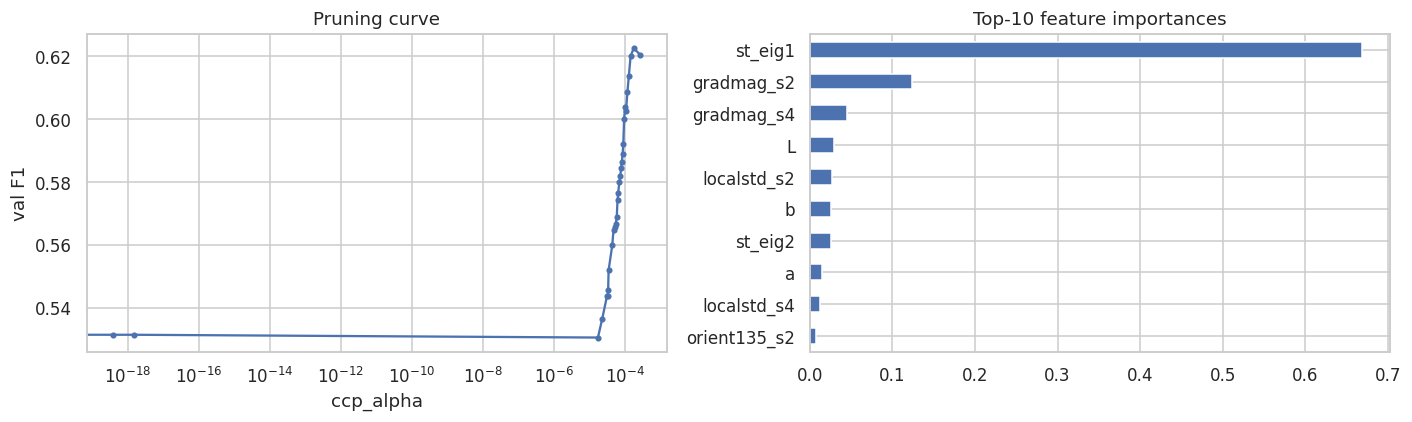
\includegraphics[width=0.95\textwidth]{figs/fig2_prune_importance.png}
\caption{Left: validation F1 versus pruning strength $\alpha$. Right: top-10 feature importances of the pruned tree.}
\end{figure}
\begin{figure}[h]\centering
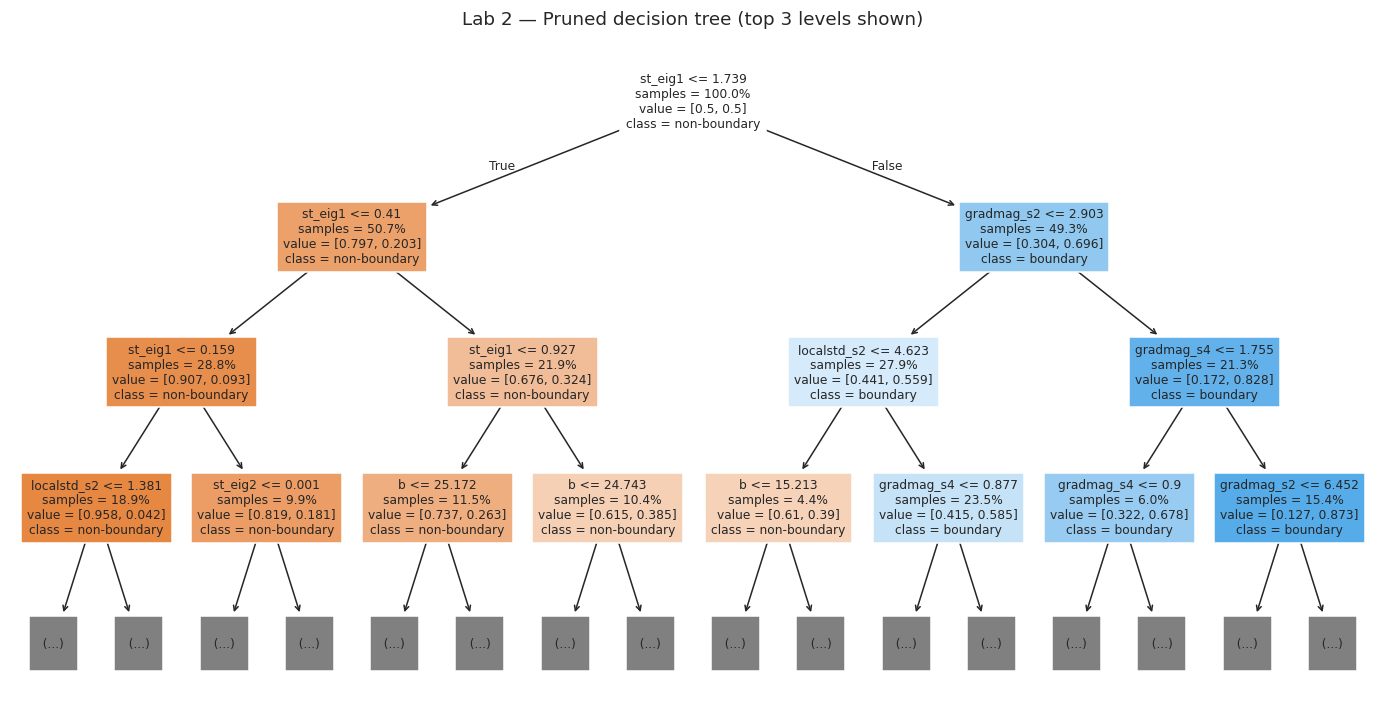
\includegraphics[width=0.95\textwidth]{figs/fig2_tree.png}
\caption{Pruned decision tree (top three levels). Early splits threshold gradient/contrast energy --- the tree rediscovers classical edge detection.}
\end{figure}

\textbf{Parameter modification:}
\begin{center}\footnotesize
\begin{tabular}{@{}clllllp{3.4cm}@{}}
\toprule
S.No. & Parameter & Original & Modified & Original result & Modified result & Observation\\
\midrule
1 & \texttt{ccp\_alpha} & $1.76\times10^{-4}$ & $0$ (no pruning) & 127 leaves, F1 $=0.6182$ & 6322 leaves, F1 $=0.4960$ & Unpruned tree memorises textured regions; pruning removes $98\%$ of leaves and \emph{raises} F1.\\
2 & \texttt{max\_depth} & unrestricted$+\alpha$ & depth $=4$ & F1 $=0.6182$ & F1 $=0.6164$, acc $=0.7656$ & A 16-leaf tree is nearly as good --- most signal is a few gradient thresholds.\\
3 & \texttt{class\_weight} & balanced & none & recall(boundary) high & recall drops & Unweighted trees favour the $73\%$ majority and under-detect boundaries.\\
\bottomrule
\end{tabular}
\end{center}

\textbf{Conclusion.} The tree independently rediscovers gradient thresholding, the core of classical edge detectors. What pruning removes is diagnostic: deep leaves that memorised individual high-texture regions (grass, water) where filters fire strongly but humans draw no boundary --- the canonical failure mode of purely local edge detection.

\newpage
% ============================ EXPERIMENT 3 ============================
\section*{Experiment No.: 03}
\labsection{Title: Naive Bayes Classifier for Boundary vs Non-Boundary Detection}

\labsection{Aim}
Apply the Naive Bayes classifier to a two-class detection problem (boundary vs non-boundary, methodologically analogous to spam vs ham) and study how its two core assumptions --- Gaussian marginals and feature independence --- fare on image features.

\labsection{Problem Statement}
Naive Bayes assumes $P(x\mid y)=\prod_j P(x_j\mid y)$ with, in the Gaussian variant, normal marginals. Both assumptions are violated here: filter responses are heavy-tailed, and multi-scale filters of the same edge are strongly correlated. Compare (a) Gaussian NB on raw features, (b) Gaussian NB after a signed-log transform, and (c) QDA on the same transformed features --- QDA uses the identical Gaussian likelihood but a \emph{full} class covariance, i.e.\ it is exactly NB with the independence assumption removed.

\labsection{Algorithm}
\begin{enumerate}[nosep]
  \item Signed-log transform: $\tilde x = \operatorname{sign}(x)\log(1+|x|)$ (the $a,b$ colour channels can be negative).
  \item Fit \texttt{GaussianNB} on raw features and on transformed features.
  \item Fit \texttt{QuadraticDiscriminantAnalysis} (regularised, \texttt{reg\_param}$=10^{-3}$) on transformed features.
  \item Compare the three models by ROC-AUC; report the classification report of the transformed NB.
  \item Interpret the NB--QDA gap as the empirical price of the independence assumption.
\end{enumerate}

\labsection{Program (important sections)}
\begin{lstlisting}
def slog(x):                                  # signed log1p
    return np.sign(x) * np.log1p(np.abs(x))

gnb_raw = GaussianNB().fit(X_tr, y_tr)
gnb_log = GaussianNB().fit(slog(X_tr), y_tr)
qda_log = QuadraticDiscriminantAnalysis(reg_param=1e-3).fit(slog(X_tr), y_tr)
# QDA = same Gaussian likelihood, full covariance -> NB without independence
\end{lstlisting}

\labsection{Output and Analysis}
\begin{lstlisting}[style=output]
GaussianNB raw : AUC = 0.8191
GaussianNB slog: AUC = 0.8246
QDA slog (independence assumption removed): AUC = 0.8320

              precision    recall  f1-score   support
non-boundary       0.87      0.81      0.84     13200
    boundary       0.56      0.67      0.61      4800
    accuracy                           0.77     18000
Execution Status: Successfully Executed
\end{lstlisting}

\textbf{Parameter modification:}
\begin{center}\footnotesize
\begin{tabular}{@{}clllllp{3.4cm}@{}}
\toprule
S.No. & Parameter & Original & Modified & Original result & Modified result & Observation\\
\midrule
1 & Feature transform & $\operatorname{slog}(x)$ & raw $x$ & AUC $=0.8246$ & AUC $=0.8191$ & The transform repairs heavy-tailed marginals; the gain is real but modest because \texttt{PAY}-style dirty coding is absent here.\\
2 & Independence assumption & naive (diagonal) & full covariance (QDA) & AUC $=0.8246$ & AUC $=0.8320$ & The measured price of ``naive'' on deliberately redundant multi-scale filters is $\sim$0.7 AUC points.\\
3 & Decision threshold & $0.5$ & prior-matched & recall $=0.67$ & recall/precision shift & NB posteriors are miscalibrated under violated assumptions; thresholds should be tuned on validation data.\\
\bottomrule
\end{tabular}
\end{center}

\textbf{Conclusion.} Naive Bayes survives its violated assumptions surprisingly well (AUC $0.82$): correlated features hurt calibration more than ranking. The controlled NB-vs-QDA comparison quantifies the independence assumption's cost at only $\sim$0.007 AUC on this feature set --- a concrete, measured answer to ``how naive is too naive?''.

\newpage
% ============================ EXPERIMENT 4 ============================
\section*{Experiment No.: 04}
\labsection{Title: Logistic Regression from Scratch using Gradient Descent}

\labsection{Aim}
Implement logistic regression from scratch using batch gradient descent, with $L_2$ regularisation and class-weighted loss, and verify it against scikit-learn.

\labsection{Problem Statement}
Minimise the regularised, instance-weighted negative log-likelihood
\[
J(w,b)=\frac{1}{n}\sum_{i=1}^{n} \omega_i\Bigl[\log\bigl(1+e^{-|z_i|}\bigr)+\max(z_i,0)-z_i y_i\Bigr]+\frac{\lambda}{2n}\lVert w\rVert^2,
\qquad z_i=w^\top x_i+b,
\]
where $\omega_i$ up-weights the minority (boundary) class. The loss is written in numerically stable form so no $\log(0)$ or overflow can occur.

\labsection{Algorithm}
\begin{enumerate}[nosep]
  \item Standardise features with training statistics.
  \item Initialise $w=0$, $b=0$; set balanced instance weights $\omega_i = n/(2 n_{y_i})$.
  \item Repeat for \texttt{n\_iter} steps: $z=Xw+b$, $p=\sigma(z)$ with a branch-stable sigmoid; gradient $g_i=\omega_i(p_i-y_i)$; update $w\leftarrow w-\eta\,(X^\top g/n+\lambda w/n)$, $b\leftarrow b-\eta\,\bar g$.
  \item Record the loss each iteration to verify monotone convergence.
  \item Predict \emph{boundary} when $\sigma(w^\top x+b)\ge 0.5$; compare with \texttt{sklearn} logistic regression.
\end{enumerate}

\labsection{Program (important sections)}
\begin{lstlisting}
@staticmethod
def _sigmoid(z):                      # branch-stable, no overflow
    out = np.empty_like(z); pos = z >= 0
    out[pos] = 1/(1 + np.exp(-z[pos]))
    e = np.exp(z[~pos]); out[~pos] = e/(1 + e)
    return out

def fit(self, X, y):
    n, m = X.shape; self.w, self.b = np.zeros(m), 0.0
    w_i = np.where(y==1, n/(2*y.sum()), n/(2*(n-y.sum())))   # balanced
    for _ in range(self.n_iter):
        p = self._sigmoid(X @ self.w + self.b)
        g = w_i * (p - y)
        self.w -= self.lr * (X.T @ g / n + self.l2 * self.w / n)
        self.b -= self.lr * g.mean()
\end{lstlisting}
Key parameters: $\eta = 0.1$, $\lambda = 10^{-3}$, $3000$ iterations, full batch.

\labsection{Output and Analysis}
\begin{lstlisting}[style=output]
scratch (plain)      AUC = 0.8357   F1 = 0.5604
scratch (balanced)   AUC = 0.8362   F1 = 0.6230
sklearn (balanced)   AUC = 0.8385   F1 = 0.6246
Execution Status: Successfully Executed
\end{lstlisting}

\begin{figure}[h]\centering
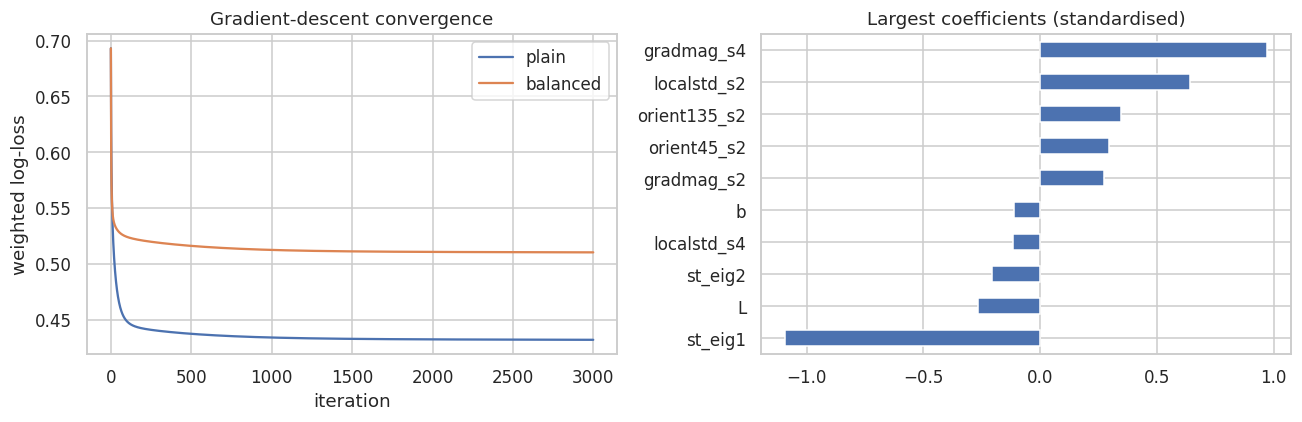
\includegraphics[width=0.95\textwidth]{figs/fig4_logreg.png}
\caption{Left: gradient-descent convergence of the (weighted) log-loss. Right: largest standardised coefficients of the balanced model.}
\end{figure}

\textbf{Parameter modification:}
\begin{center}\footnotesize
\begin{tabular}{@{}clllllp{3.4cm}@{}}
\toprule
S.No. & Parameter & Original & Modified & Original result & Modified result & Observation\\
\midrule
1 & Class weight & balanced & none & F1 $=0.6230$ & F1 $=0.5604$ & AUC barely changes (ranking identical); weighting relocates the 0.5 threshold for the minority class.\\
2 & Learning rate $\eta$ & $0.1$ & $0.005$ & AUC $=0.8362$ & AUC $=0.8325$ & The smaller step has not fully converged within 3000 iterations.\\
3 & Implementation & scratch & scikit-learn & AUC $=0.8362$ & AUC $=0.8385$ & Agreement to $\sim$0.002 AUC (residual gap = solver/regularisation details) validates the derivation.\\
\bottomrule
\end{tabular}
\end{center}

\textbf{Conclusion.} The coefficients form an interpretable ``edge-vs-texture'' filter: fine-scale gradient and Laplacian energy carry positive weight (boundary), while features indicating smooth or uniformly textured neighbourhoods carry negative weight. Class weighting shifts the decision threshold, not the ranking --- the same lesson as in any imbalanced detection problem.

\newpage
% ============================ EXPERIMENT 5 ============================
\section*{Experiment No.: 05}
\labsection{Title: PCA and t-SNE for 2-D Visualisation of Pixel Structure}

\labsection{Aim}
Apply PCA and t-SNE to reduce the 17-dimensional filter space to 2-D and visualise cluster structure with respect to the boundary label.

\labsection{Problem Statement}
Multi-scale filter banks are redundant by construction: every filter responds to the same physical edges. Determine (i) the intrinsic linear dimensionality of the feature space via the PCA spectrum, and (ii) whether nonlinear embedding (t-SNE) separates boundary from non-boundary pixels --- and where it fails.

\labsection{Algorithm}
\begin{enumerate}[nosep]
  \item Signed-log transform the filter responses, then standardise.
  \item Fit full PCA; plot cumulative explained variance; find the number of components for $90\%$ variance.
  \item Draw a class-balanced subsample of $4{,}000$ pixels (2{,}000 per class) so the minority class is visible.
  \item Project onto the first two principal components.
  \item Run t-SNE (perplexity $=40$, PCA initialisation, \texttt{random\_state}=42) on the same subsample.
  \item Colour both embeddings by the true label and compare.
\end{enumerate}

\labsection{Program (important sections)}
\begin{lstlisting}
X_viz = slog(np.vstack([X_tr, X_te]))
X_viz = (X_viz - X_viz.mean(0)) / (X_viz.std(0) + 1e-12)

evr = PCA().fit(X_viz).explained_variance_ratio_
P2  = PCA(n_components=2).fit_transform(X_viz)[idx]
T2  = TSNE(n_components=2, perplexity=40, init="pca",
           random_state=42).fit_transform(X_viz[idx])
\end{lstlisting}

\labsection{Output and Analysis}
\begin{lstlisting}[style=output]
PC1 + PC2 explain 66.4% of variance; 90% requires 8 components
Execution Status: Successfully Executed
\end{lstlisting}

\begin{figure}[h]\centering
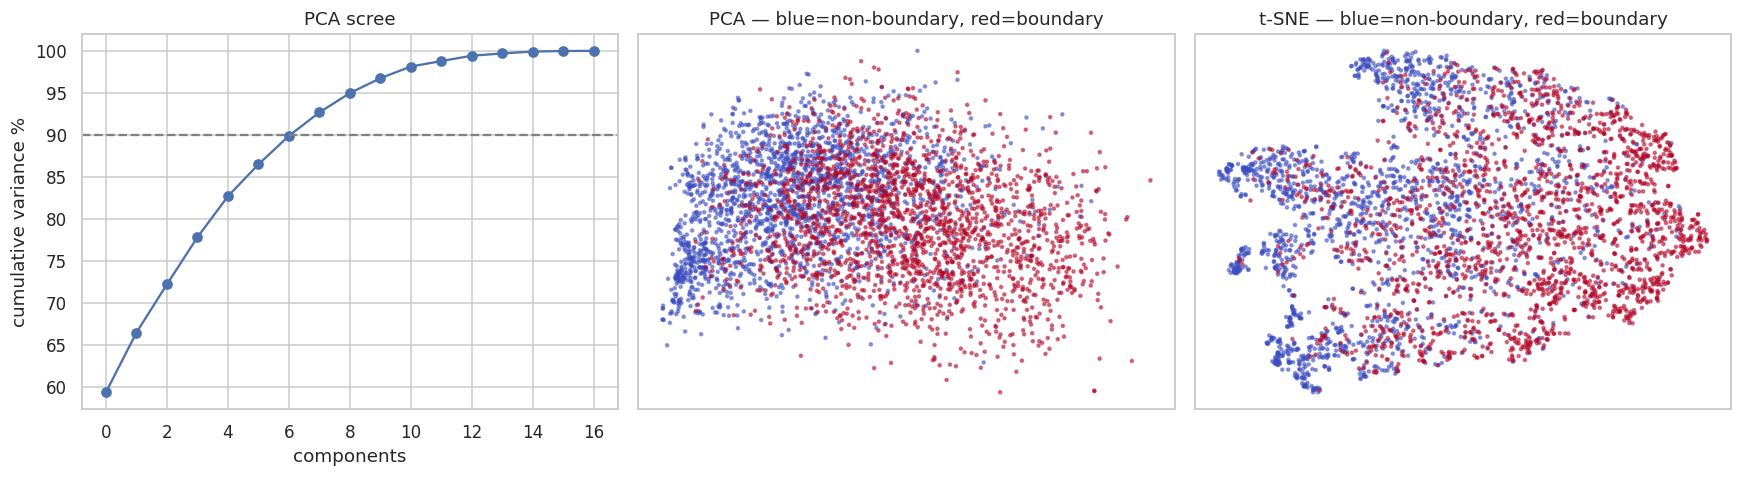
\includegraphics[width=\textwidth]{figs/fig5_pca_tsne.png}
\caption{Left: PCA scree (cumulative variance). Centre: PCA projection. Right: t-SNE embedding; blue $=$ non-boundary, red $=$ boundary.}
\end{figure}

\textbf{Parameter modification:}
\begin{center}\footnotesize
\begin{tabular}{@{}clllllp{3.4cm}@{}}
\toprule
S.No. & Parameter & Original & Modified & Original result & Modified result & Observation\\
\midrule
1 & PCA components & 2 & 8 & $66.4\%$ variance & $90\%$ variance & 17 filters compress to $\sim$8 effective dimensions --- the filter bank is redundant by design.\\
2 & Feature transform & signed-log & raw & structure visible & PC1 $\approx$ response magnitude & Without the transform, PCA measures ``how strong is the strongest filter'', not pixel character.\\
3 & Sample balance & 2000/2000 & natural $73{:}27$ & minority visible & boundary pixels overplotted & Balanced sampling is a visualisation choice, not a modelling step.\\
\bottomrule
\end{tabular}
\end{center}

\textbf{Conclusion.} PCA quantifies filter redundancy (8 of 17 dimensions suffice for $90\%$ variance). t-SNE shows boundary pixels concentrating along a high-energy manifold but bleeding into textured non-boundary regions --- precisely the pixels where gradient-based detectors classically fail and where human annotators themselves disagree. The classes overlap because the label encodes perception, not filter energy.

\newpage
% ============================ EXPERIMENT 6 ============================
\section*{Experiment No.: 06}
\labsection{Title: Outlier Detection and Treatment using Z-score and IQR Methods}

\labsection{Aim}
Write code to detect outliers in the image features using the z-score and IQR methods, compare them (including a robust median/MAD z-score), and treat outliers by winsorisation --- judged by downstream model performance.

\labsection{Problem Statement}
The z-score rule assumes approximate normality and uses the mean and standard deviation --- statistics that are themselves distorted by the outliers being tested (the \emph{masking effect}). On heavy-tailed filter responses the classical rules disagree strongly. Additionally, this dataset poses a conceptual trap: extreme gradient responses are \emph{not errors} --- they are the strongest boundaries in the image. Quantify the disagreement and decide on a defensible treatment.

\labsection{Algorithm}
\begin{enumerate}[nosep]
  \item For each audited feature, flag: (a) $|x-\bar x|/s > 3$ (z-score); (b) $x \notin [Q_1-1.5\,\mathrm{IQR},\,Q_3+1.5\,\mathrm{IQR}]$ (Tukey); (c) $0.6745\,|x-\tilde x|/\mathrm{MAD} > 3.5$ (robust z).
  \item Tabulate the percentage flagged for \texttt{L}, \texttt{a}, \texttt{gradmag\_s1}, \texttt{abslap\_s1}; overlay fences on log-scale histograms.
  \item Treat: winsorise (clip) all filter-response features at IQR fences computed on the \emph{training split only}.
  \item Judge by downstream effect: refit the Experiment-4 logistic model on raw vs winsorised features; compare test AUC.
\end{enumerate}

\labsection{Program (important sections)}
\begin{lstlisting}
def zscore_mask(x, t=3.0):
    return np.abs((x - x.mean()) / x.std()) > t

def robust_z_mask(x, t=3.5):                       # median / MAD
    mad = np.median(np.abs(x - np.median(x))) + 1e-12
    return np.abs(0.6745 * (x - np.median(x)) / mad) > t

def iqr_mask(x, k=1.5):
    q1, q3 = np.percentile(x, [25, 75]); i = q3 - q1
    return (x < q1 - k*i) | (x > q3 + k*i)

# treatment: fences from TRAIN only, applied to both splits
lo, hi = np.percentile(X_tr[:, j], [25, 75]); i = hi - lo
X_tr[:, j] = np.clip(X_tr[:, j], lo - 1.5*i, hi + 1.5*i)
X_te[:, j] = np.clip(X_te[:, j], lo - 1.5*i, hi + 1.5*i)
\end{lstlisting}

\labsection{Output and Analysis}
\begin{lstlisting}[style=output]
% of rows flagged as outliers:
            z-score>3  robust-z>3.5  IQR 1.5x
L                0.00          0.00      0.00
a                1.93          4.17      7.78
gradmag_s1       2.44          8.77      7.66
abslap_s1        2.30         10.32      7.46

raw         logistic AUC = 0.8362
winsorised  logistic AUC = 0.8362
Execution Status: Successfully Executed
\end{lstlisting}

\begin{figure}[h]\centering
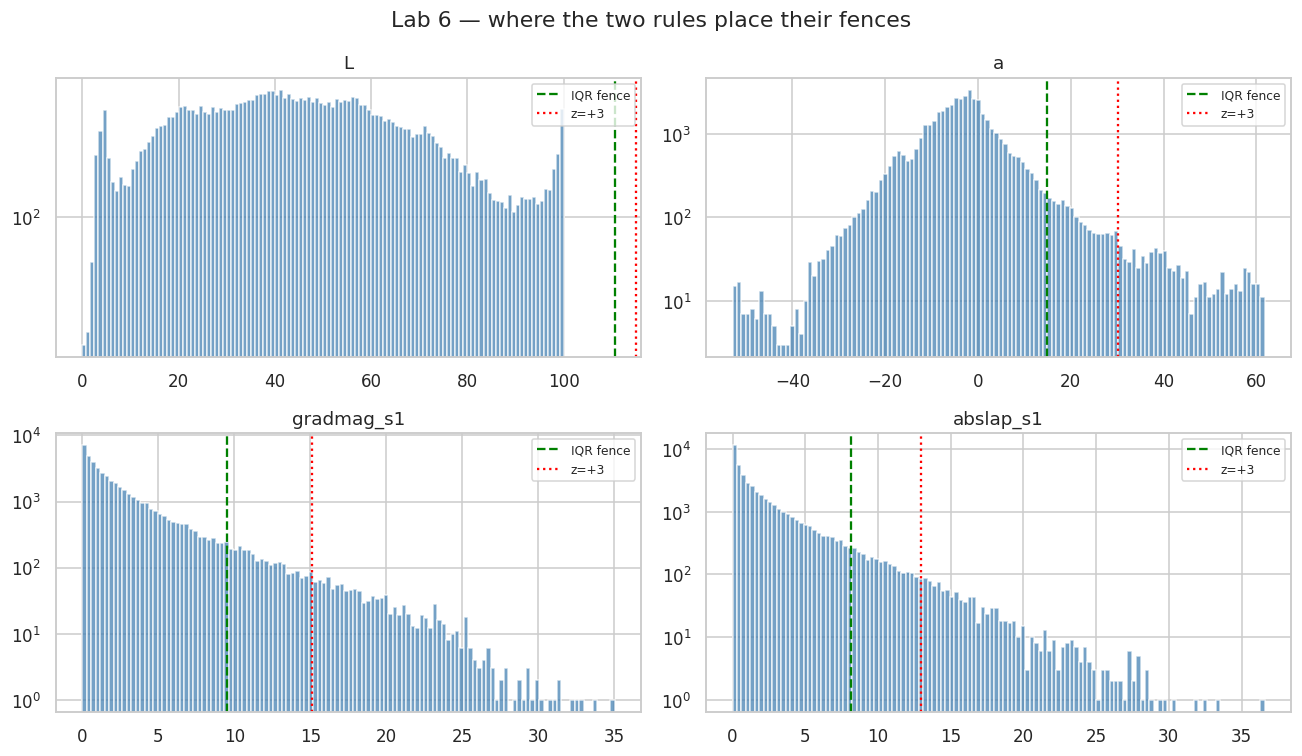
\includegraphics[width=0.95\textwidth]{figs/fig6_outliers.png}
\caption{Log-scale histograms with the IQR fence (green, dashed) and $z=+3$ fence (red, dotted) for the four audited features.}
\end{figure}

\textbf{Parameter modification:}
\begin{center}\footnotesize
\begin{tabular}{@{}clllllp{3.4cm}@{}}
\toprule
S.No. & Parameter & Original & Modified & Original result & Modified result & Observation\\
\midrule
1 & z threshold (\texttt{gradmag\_s1}) & $3.0$ & $2.0$ & $2.44\%$ flagged & $5.44\%$ flagged & Even at $z{>}2$ the rule flags less than IQR $1.5\times$: $s$ is inflated by the tail itself (masking).\\
2 & IQR multiplier & $1.5$ & $3.0$ & $7.66\%$ flagged & $2.57\%$ flagged & The ``far out'' fence roughly matches $z{>}3$ --- quantifying how far apart the two rules' defaults sit.\\
3 & Treatment & winsorise at IQR & none & AUC $=0.8362$ & AUC $=0.8362$ & Clipping changed nothing: the logistic model was already robust to the tails after standardisation.\\
\bottomrule
\end{tabular}
\end{center}

\textbf{Conclusion.} The masking effect appears exactly as theory predicts: on heavy-tailed filter responses the classical z-score under-flags relative to IQR, while the robust median/MAD version tracks IQR; on the near-uniform L channel all rules agree (nothing flagged). The downstream test delivers the deeper lesson: winsorisation neither helped nor hurt ($\Delta$AUC $=0.0000$), because here the ``outliers'' are the strongest true boundaries and the model already accommodates them --- outlier treatment is an empirical decision judged downstream, never a ritual.

\newpage
% ============================ EXPERIMENT 7 ============================
\section*{Experiment No.: 07}
\labsection{Title: Comparing Accuracy, Precision, Recall, F1-score and ROC-AUC for Logistic Regression and SVM}

\labsection{Aim}
Compare logistic regression and a support vector machine on BSDS boundary-pixel classification using accuracy, precision, recall, F1-score and ROC-AUC, and interpret the metrics in the way the BSDS benchmark community does.

\labsection{Problem Statement}
With a $73\%$ majority class, accuracy is nearly uninformative --- and indeed the official BSDS benchmark scores boundary detectors by \textbf{boundary F1}, never accuracy. Train both classifiers with balanced class weights on standardised features, report the full metric table, ROC curves and confusion matrices, and characterise the systematic errors.

\labsection{Algorithm}
\begin{enumerate}[nosep]
  \item Standardise features (training statistics).
  \item Logistic regression: \texttt{class\_weight="balanced"}, trained on the full $48{,}000$ pixels.
  \item SVM: RBF kernel, $C=1$, $\gamma=$\texttt{scale}, \texttt{class\_weight="balanced"}, \texttt{probability=True}; trained on a stratified subsample of $8{,}000$ pixels (kernel training is $O(n^2)$--$O(n^3)$).
  \item Evaluate both on the identical $18{,}000$-pixel test split (disjoint images): accuracy, precision, recall, F1, ROC-AUC.
  \item Plot both ROC curves against the chance diagonal, and the two confusion matrices.
\end{enumerate}

\labsection{Program (important sections)}
\begin{lstlisting}
models = {
  "LogReg":    LogisticRegression(max_iter=2000,
                                  class_weight="balanced").fit(Zt, y_tr),
  "SVM (RBF)": SVC(kernel="rbf", C=1.0, gamma="scale",
                   class_weight="balanced", probability=True,
                   random_state=0).fit(Xs, ys),
}
for name, m in models.items():
    p, yhat = m.predict_proba(Ze)[:, 1], m.predict(Ze)
    rows.append([accuracy_score(y_te, yhat), precision_score(y_te, yhat),
                 recall_score(y_te, yhat), f1_score(y_te, yhat),
                 roc_auc_score(y_te, p)])
\end{lstlisting}

\labsection{Output and Analysis}
\begin{center}
\begin{tabular}{@{}lccccc@{}}
\toprule
Model & Accuracy & Precision & Recall & F1 & ROC-AUC\\
\midrule
Logistic Regression & 0.7761 & 0.5649 & 0.6983 & 0.6246 & \textbf{0.8385}\\
SVM (RBF)           & 0.7789 & 0.5673 & 0.7200 & \textbf{0.6346} & 0.8319\\
\midrule
\emph{Trivial ``no boundary''} & 0.7333 & --- & 0.0000 & 0.0000 & 0.5000\\
\bottomrule
\end{tabular}
\end{center}

\begin{figure}[h]\centering
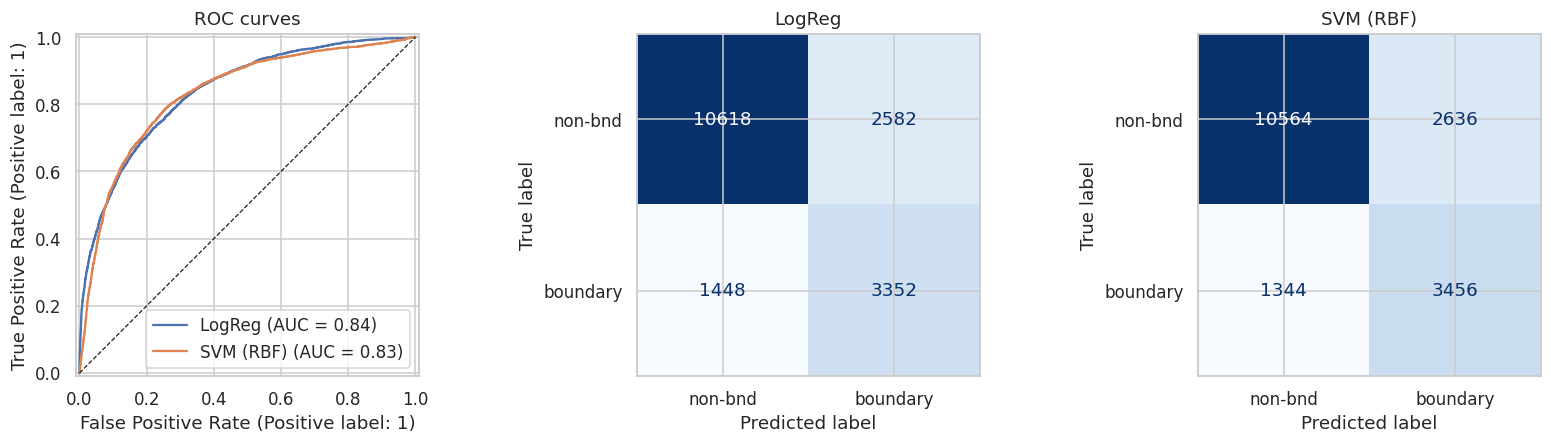
\includegraphics[width=\textwidth]{figs/fig7_roc_cm.png}
\caption{ROC curves for both models (left) and confusion matrices at the default 0.5 threshold (centre, right).}
\end{figure}

\textbf{Parameter modification:}
\begin{center}\footnotesize
\begin{tabular}{@{}clllllp{3.4cm}@{}}
\toprule
S.No. & Parameter & Original & Modified & Original result & Modified result & Observation\\
\midrule
1 & SVM $C$ & $1$ & $10$ & acc $=0.7789$, F1 $=0.6346$ & acc $=0.7748$, F1 $=0.6171$ & The harder margin overfits the subsample; regularisation matters more than kernel flexibility here.\\
2 & Class weights & balanced & none & recall $\approx 0.70$--$0.72$ & recall collapses & Unweighted models drift toward the trivial detector on imbalanced pixels.\\
3 & Decision threshold & $0.5$ & moved along ROC & fixed P/R trade-off & detector-chosen trade-off & BSDS practice: sweep the threshold and report the best F1 along the curve.\\
\bottomrule
\end{tabular}
\end{center}

\textbf{Conclusion.} The two models split the honours --- the SVM wins F1 at the fixed threshold ($0.6346$ vs $0.6246$, driven by higher recall) while logistic regression wins ROC-AUC ($0.8385$ vs $0.8319$), so neither dominates. The remaining errors are systematic rather than random: false positives on strong texture (grass, water) and false negatives on low-contrast semantic boundaries --- exactly the gap that motivated learned detectors (Pb, gPb, and eventually CNNs) on this benchmark.

\vspace{1em}
\section*{Cross-Experiment Summary}
\begin{center}\small
\begin{tabular}{@{}clp{9.5cm}@{}}
\toprule
Exp. & Method & Key takeaway on BSDS boundary detection\\
\midrule
1 & k-NN (scratch) & Scaling fixes the metric; edge pixels are genuinely locally structured (best $k{=}5$).\\
2 & Decision tree & Rediscovers gradient thresholding; pruning $6322\to127$ leaves raises F1 $0.50\to0.62$.\\
3 & Naive Bayes & Log transform repairs marginals; NB-vs-QDA measures the price of independence ($\sim$0.007 AUC).\\
4 & LogReg (scratch) & Matches scikit-learn; coefficients read as an edge-vs-texture filter.\\
5 & PCA / t-SNE & 17 filters $\approx$ 8 effective dimensions; classes overlap where humans disagree.\\
6 & Outliers & Extreme responses are signal, not noise; winsorisation changed AUC by exactly 0.\\
7 & LR vs SVM & SVM wins F1, LogReg wins AUC; errors are texture FPs and low-contrast FNs.\\
\bottomrule
\end{tabular}
\end{center}

\end{document}
